\documentclass[]{article}

\usepackage[utf8]{inputenc}
\usepackage[english,serbian]{babel}
\usepackage[margin=0.7in]{geometry}
\usepackage{url}
\usepackage{float}
\usepackage[graphicx]{realboxes}
\usepackage{listings}
\usepackage{textcomp}
\usepackage{xcolor}
\usepackage{titlesec}
\usepackage{adjustbox}
\lstset {
    language=HTML,
    frame=none,
    %xleftmargin=-.25in,
    %xrightmargin=.25in
    framesep=10pt,
    tabsize=4,
    showstringspaces=false,
    upquote=true,
    commentstyle=\color{black},
    keywordstyle=\color{black},
    stringstyle=\color{black},
    basicstyle=\small\ttfamily,
    emph={int,char,double,float,unsigned,void,bool},
    emphstyle={\color{black}},
    escapechar=\&,
    classoffset=1,
    morekeywords={>,<,.,;,,,-,!,=,~},
    keywordstyle=\color{black},
    classoffset=0,
    breaklines=true
}
\pagenumbering{gobble}

\titlespacing\title{left spacing}{before spacing}{after spacing}[right]

\title{Ra\v{c}unarske mre\v{z}e 4R, Ispit - Jun 1}
\date{14.06.2019.}

\begin{document}

\makeatletter
\begin{center}

{\fontsize{12pt}{14pt}\selectfont\bfseries\@title\par}
\@date

Pro\v{c}itati sve zadatke \textbf{pa\v{z}ljivo} pre rada - sve \v{s}to nije navedeno ne mora da se implementira! 

Vreme za rad: \textbf{2.5h}. Sre\'{c}no!
\end{center}
\makeatother


\begin{enumerate}
  \item Sockets \textbf{(15p)}
  \begin{itemize}
    \item Napraviti Java aplikaciju koja ima ulogu UDP servera. Slu\v{s}ati na portu 12345 i primiti pakete od klijenata koriste\'c{}i \texttt{DatagramPacket} klasu. Sadr\v{z}aj svakog paketa treba da je velicine \texttt{4B}. Ispisati tekst \texttt{Stigao paket!} kad god server primi validan paket od nekog klijenta. \hfill (3p)
    \item Napraviti Java aplikaciju koja ima ulogu UDP klijenta. Poslati UDP paket lokalnom serveru na portu 12345 koriste\'c{}i \texttt{DatagramPacket} klasu. Sadr\v{z}aj svakog paketa je jedan pozitivan ceo broj veli\v{c}ine \texttt{4B}. \hfill (3p)
    \item Promeniti implementaciju klijenta tako da u petlji $n$ puta ($n$ se unosi sa standardnog ulaza) \v{s}alje pakete serveru sa nasumi\v{c}no izabranim pozitivnim celim brojem manjim od $1000$ kao sadr\v{z}ajem. \hfill (3p)
    \item Server pamti i a\v{z}urira promenljivu \texttt{S} (inicijalna vrednost $0$) tako \v{s}to sadr\v{z}aj svakog validnog primljenog paketa dodaje na vrednost promenljive \texttt{S}. Server na svakih $5$ primljenih validnih paketa ispisuje trenutnu vrednost promenljive \texttt{S}. \hfill (3p)
    \item Implementirati odgovor od servera klijentu koji je poslao paket. Klijent \v{s}alje slede\'c{}i paket tek kada od servera dobije potvrdu da je primljen paket (ignorisati verovatno\'c{}u gubitka paketa). \hfill (2p)
    \item Postarati se da su svi resursi ispravno zatvoreni u slu\v{c}aju izuzetka. \hfill (1p)
  \end{itemize}

  \item Swing \textbf{(15p)}
  Napraviti Java Swing aplikaciju koja ima ulogu jednostavnog HTML editora. Izgled aplikacije je dat na slici ispod.
  \begin{itemize}
    \item Ispo\v{s}tovati izgled aplikacije (ne me\v{s}ati redosled komponenti i postarati se da su odnosi u veli\v{c}ini kao na slici). \hfill (2p)
    \item Napraviti prozor i u njega dodati skrolabilnu komponentu za prikaz sadr\v{z}aja tekstualnog fajla. \hfill (2p)
    \item Omogu\'c{}iti da se prozor mo\v{z}e pro\v{s}iriti i smanjiti a da se raspored i razmera komponenti ne promeni. \hfill (2p)
    \item Dodati komponentu za unos URL-a koji vodi do HTML fajla (testirati na lokalnom fajl-sistemu koriste\'c{}i FILE protokol). Dodati dugme \texttt{Prika\v{z}i} koje dovla\v{c}i HTML fajl sa datog URL-a prikazuje sadr\v{z}aj tog fajla u komponenti za prikaz. Ako URL nije validan ili ne vodi do HTML fajla, dugme ne radi ni\v{s}ta. \hfill (4p)
    \item Dodati dugme \texttt{Sa\v{c}uvaj} \v{c}iji je efekat da sa\v{c}uva izmene HTML fajla koriste\'c{}i izlazni \texttt{Stream} do fajla sa putanjom iz komponente za unos URL-a. \hfill (4p)
  \end{itemize}

  \begin{figure}[H]
    \centering
    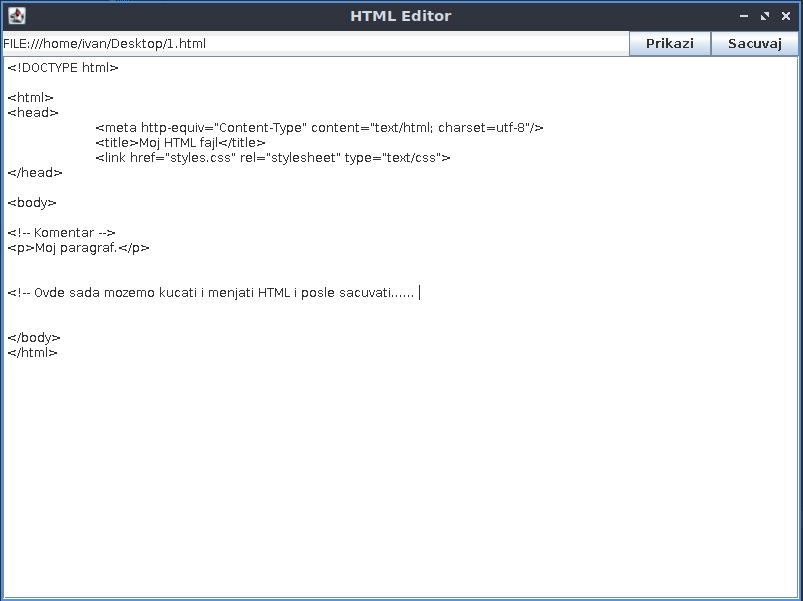
\includegraphics[scale=0.6]{fig.PNG}
    \label{fig2}
  \end{figure}
\end{enumerate}

\end{document}
